\addtocontents{toc}{\protect\setcounter{tocdepth}{1}}
\chapter*{APÊNDICE B - DOCUMENTO DE PERSONAS}\label{apendice_personas}
\addcontentsline{toc}{chapter}{APÊNDICE B - DOCUMENTO DE PERSONAS}
\addtocontents{toc}{\protect\setcounter{tocdepth}{-1}}

\section{Charlie - Técnico em Informática}

\begin{figure}[H]
\centering
\caption{Imagem de Charlie}

\includegraphics[width=5cm]{figuras/personas/figura_persona_1}
\fnote{Fonte: \url{www.geradordepersonas.com.br} }
\label{figura_persona_1}
\end{figure}


Empresa: Charlie trabalha na TechSolutions, uma empresa de tecnologia pequena, mas que está ganhando
clientes e ampliando seus negócios.

Idade: 24 anos.

Genêro: Masculino.

Educação: Ensino técnico.

Mídias: Lê a revista Exame e usa ativamente email para trocar informações com 
outros funcionários da empresa.

Objetivos: Como a empresa que Charlie trabalha está ampliando seus negócios, ela
necessita que alguns de seus funcionários possuam um melhor conhecimento na 
área, por isso, Charlie decidiu investir num ensino superior. O objetivo de Charlie é 
concluir seu curso de Engenharia de Software e voltar a trabalhar normalmente 
para sua empresa.

Desafios: Charlie está com muita dificuldade na primeira disciplina de Matemática de seu curso. Como ele já concluiu o ensino médio há bastante tempo, ele não se lembra de como resolver 
questões simples de matemática como funções de 1º grau, 2º grau, racionais, entre outras. Ele começou a estudar, mas 
não consegue encontrar uma forma intuitiva para verificar se está indo bem nos 
seus estudos, ficando preso aos exercícios que ele encontra nos livros.

Como podemos ajudá-lo: O AskMath possibilitará que Charlie estude 
todos os conteúdos que ele j\'a havia estudado no ensino médio e que já os tinha esquecido. São lições agrupadas por disciplina, cada lição possui um conjunto de problemas criados especialmente para 
pessoas com dificuldade em aprender. Nosso sistema possibilitará que Charlie veja instantaneamente se sua resposta é correta ou não, ele também poderá pedir ajuda 
e saltar quest\~oes caso o mesmo não se sinta a vontade para respondê-las naquele 
momento. Com isso, é possível que ele acompanhe através de estatísticas como 
está seu desempenho durante os estudos.

\section{Ruby - Bolsista de Graduação}

\begin{figure}[H]
\centering
\caption{Imagem de Ruby}
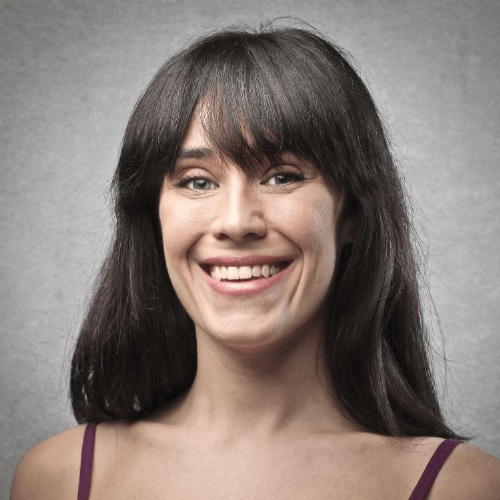
\includegraphics[width=5cm]{figuras/personas/figura_persona_2}
\fnote{Fonte: \url{www.geradordepersonas.com.br} }
\label{figura_persona_2}
\end{figure}


Empresa: Ruby trabalha como bolsista de monitoria das disciplinas envolvendo 
Matemática na Universidade Federal do Ceará.

Idade: 21 anos.

Genêro: Feminino.

Educação: Ensino superior.

Mídias: Usa ativamente o facebook, twitter e wattsapp.

Objetivos: O principal objetivo de Ruby é terminar sua graduação e tentar uma 
bolsa de mestrado numa universidade renomada.

Desafios: Ruby como monitora das disciplinas de matemática, não consegue se
aproximar dos alunos para ajuda-los com suas dúvidas. Segundo ela, "eles tem medo de 
dizer para nós monitores que est\~ao com dificuldades", então Ruby está em busca de 
novas formas de ajudar os estudantes que estão com dificuldades.

Como podemos ajudá-la: Com o AskMath, Ruby poderá ajudar esses alunos adicionando problemas para eles exercitarem seus conhecimentos e tirar suas d\'uvidas no f\'orum de discuss\~ao que 
o sistema oferece.

\section{Samuel - Professor}

\begin{figure}[H]
\centering
\caption{Imagem de Samuel}
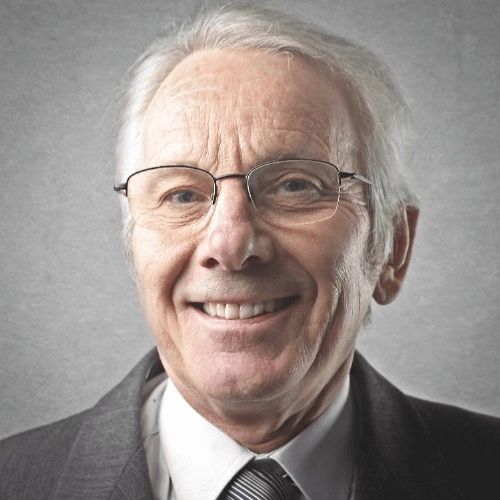
\includegraphics[width=5cm]{figuras/personas/figura_persona_3}
\fnote{Fonte: \url{www.geradordepersonas.com.br} }
\label{figura_persona_3}
\end{figure}

Empresa: Samuel trabalho como professor da disciplina de C\'alculo I na
Universidade Federal do Ceará.

Idade: 59 anos.

Genêro: Masculino.

Educação: Doutorado.

Mídias: Lê o jornal The New York Times e usa email para tirar dúvidas dos alunos.

Objetivos: Samuel é um professor exemplar e se preocupa muito em ensinar seus 
alunos. Seu principal objetivo é ensinar da melhor forma possível seus alunos, 
de forma que todos possam seguir excelentes carreiras quando se formar e se 
tornem ótimos profissionais.

Desafios: Samuel gosta de acompanhar o andamento dos estudos de seus alunos. Quando Samuel os questionam sobre as dificuldade que eles est\~ao enfrentando nos seus estudos, os mesmos dizem que ``está 
tudo bem'', o que não reflete em suas notas. Sabendo disso, Samuel fica triste, já que não consegue saber como anda os estudos de seus alunos e gostaria de ajudá-los ainda mais.

Como podemos ajudá-lo: Com o AskMath, Samuel poder\'a acompanhar o andamento de sua turma e saber em quais conteúdos os alunos est\~ao com mais dificuldade, para dar uma aten\c{c}\~ao especial a 
esses conte\'udos. Samuel poderá ainda adicionar os conteúdos que ele achar mais interessantes, para que seus alunos possam praticar os conhecimentos adquiridos em sala de aula no conforto de suas 
casas. Samuel tamb\'em ver\'a as dúvidas que os alunos postam no fórum de discuss\~oes e quais desses alunos est\~ao enfrentando obstáculos durante sua aprendizagem.

\section{Stefane - Estudante do Ensino Médio}

\begin{figure}[H]
\centering
\caption{Imagem de Stefane}
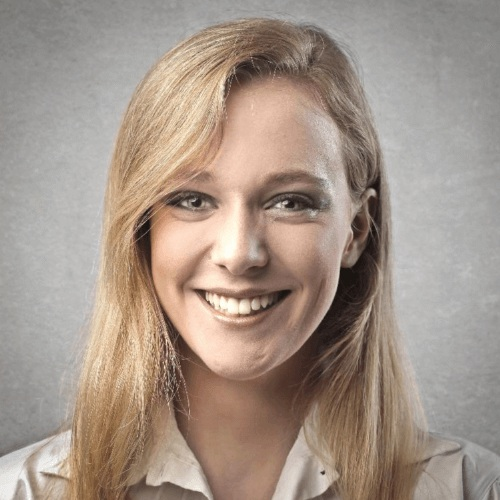
\includegraphics[width=5cm]{figuras/personas/figura_persona_4}
\fnote{Fonte: \url{www.geradordepersonas.com.br} }

\label{figura_persona_4}
\end{figure}

Empresa: Ela trabalha no salão de beleza de sua mãe.

Idade: 18 anos.

Genêro: Feminino.

Educação: Ensino médio.

Mídias: Usa ativamente o facebook e WatssApp.

Objetivos: Stefane busca concluir o ensino médio e tirar uma boa nota no ENEM 
para tentar conseguir uma vaga para cursar Sistemas de Informação na Universidade Federal do Cear\'a, que é 
o curso de seus sonhos.

Desafios: Stefane, como estudante, não gosta de estudar matemática por livros e acha incomodo ter que levar seus livros enormes de matemática em sua bolsa para o salão de beleza de sua mãe para 
estudar, mas tamb\'em quer ficar estudando enquanto não aparece clientes no salão. Um outro problema de Stefane, é que às vezes, ela fica com dúvidas na resolução de algum problema e precisa ligar 
para seus amigos em busca de explicações que nem sempre encontra.

Como podemos ajudá-la: Com o AskMath, Stefane não precisará mais levar seus livros de Matemática em sua bolsa, para aprender matemática ela precisar\'a apenas de uma celular e isso possibilita que 
ela possa continuar estudando no salão enquanto este estiver vazio. Para solucionar as dúvidas de Stefane, 
temos pessoas esperando para ajudá-la no f\'orum de discuss\~ao, em que ela pode compartilhar suas d\'uvidas para que outros estudantes e professores possam ajuda-la e ao mesmo tempo ajudar outros 
que estejam com a mesma d\'uvida de Stefane. 